%!TEX root = ../../../FYP_Dissertation.tex

%===============================================================================
% Methodical Accelerator Design
%===============================================================================

\subsection{Methodical Accelerator Design}
\label{Subsec:mad-orig}

MAD or Methodical Accelerator Design is a complete set of tools bundle together
and developed at CERN to design, study, simulate and optimize beam physics for
particle accelerators. Its current version is called MAD-X. It was first released
in 2002 and is the successor of  MAD-8 (see official website \cite{madx}).
Its source code is mainly written in C, C++, Fortan77 and Fortran90.
It presents itself as a command-line program that reads and execute its custom
scripting language. This language has the particularity of having a single
workspace where everything is global. There is no function but a simple macro
system. Most of the functionalities are provided through high-level commands that
can be customized by the user. Deferred expressions are heavily used everywhere.
This code has been internally known to
be difficult to maintain and improve. In additions of that, developing new
functionality for it takes a significant amount of time due to the fact that
module are tightly coupled and modification on its big code base can have
unexpected side effect if the developer is not careful. The need for
consolidation plus the rise of efficient and modern languages making the
development faster and more flexible triggered a new redesign of the MAD
application called MAD-NG.


%===============================================================================
% MAD-NG
%===============================================================================

\subsection{MAD Next Generation}
\label{Subsec:mad-ng}

MAD-NG or Methodical Accelerator Design Next Generation is, like stated previously,
a modern redesign of the MAD application. The objectives of MAD-NG are, to use
a simple scripting language to offer easier and faster development, to propose
a well-compartmented and modular design for scalability, to allow much more
flexible user input, to reintroduce computer science good practices with scopes,
functions, control-flow, etc.. It has to do so while being at least as performant
as MAD-X, keeping the high level command-like philosophy and staying a standalone
single binary working out of the box without any installation procedure.
The scripting language Lua through LuaJIT as been picked (see Section \ref{Sec:LuaJIT}).
Figure \ref{fig:mad-screnshot} illustrates a run of the test suite of MAD-NG on
a mac. The \emph{all.mad} file is the entry file for all tests and in this example,
we specified that we wanted to run only the \emph{Sequence} tests.

\begin{figure}[H]
    \centering
	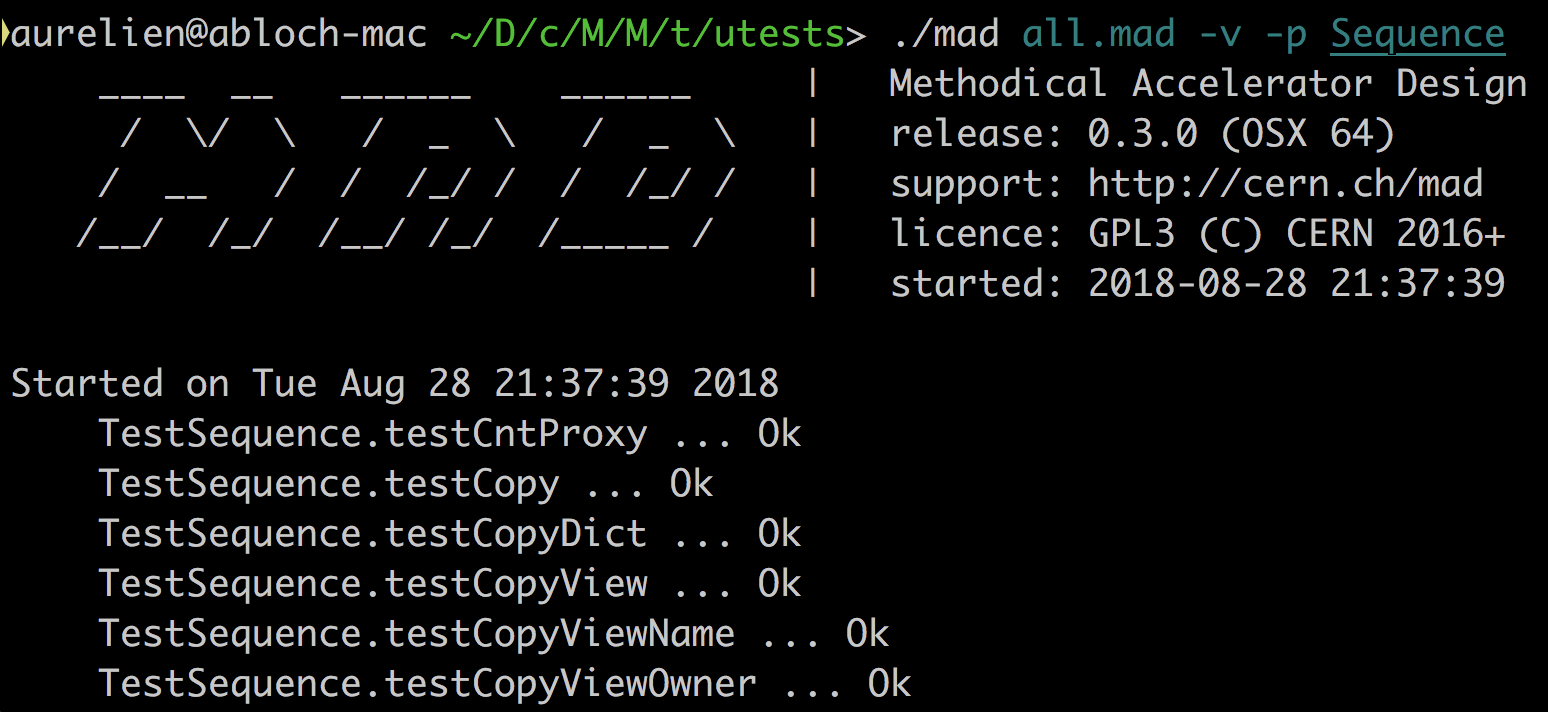
\includegraphics[width=0.8\textwidth]{./Images/mad-screenshot}
    \caption{Screenshot of a test run of MAD.}
    \label{fig:mad-screnshot}
\end{figure}

\subsubsection{MAD-NG packaging}
\label{Subsec:mad-pk}

Figure \ref{fig:mad} shows how the MAD-NG application is being packaged. Some
modifications over LuaJIT has been done to allow it to be embedded inside of MAD
as by default LuaJIT cannot be moved after being installed.
The source code of MAD is mainly implemented in Lua (\emph{*.mad} extension
files) but for performance reasons some physic calculations and algorithms are
written in \emph{C}. A big advantage of LuaJIT is the efficiency of the FFI
library (Foreign Function Interface) that allows to use embedded \emph{C} code
or even \emph{C} libraries directly inside the Lua application.

\begin{figure}[H]
    \centering
	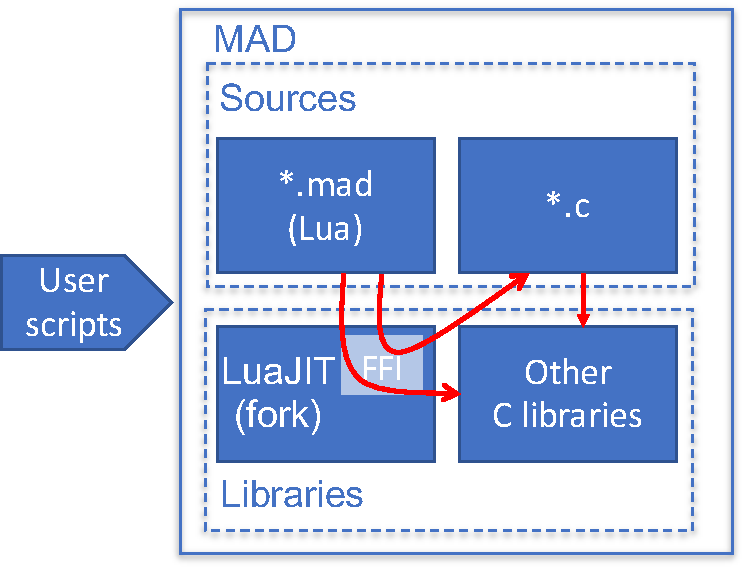
\includegraphics[width=9cm]{./Images/MAD.pdf}
    \caption{MAD-NG application}
    \label{fig:mad}
\end{figure}

\subsubsection{MAD-NG modules overview}
\label{Subsec:mad-doc}

This section does not attempt to provide a full documentation of MAD but a
minimum amount to be able to understand the rest of this dissertation.
Figure \ref{fig:mad-graph} below is a graph representing the different
modules currently available in MAD and the way they are connected.

\begin{figure}[H]
    \centering
	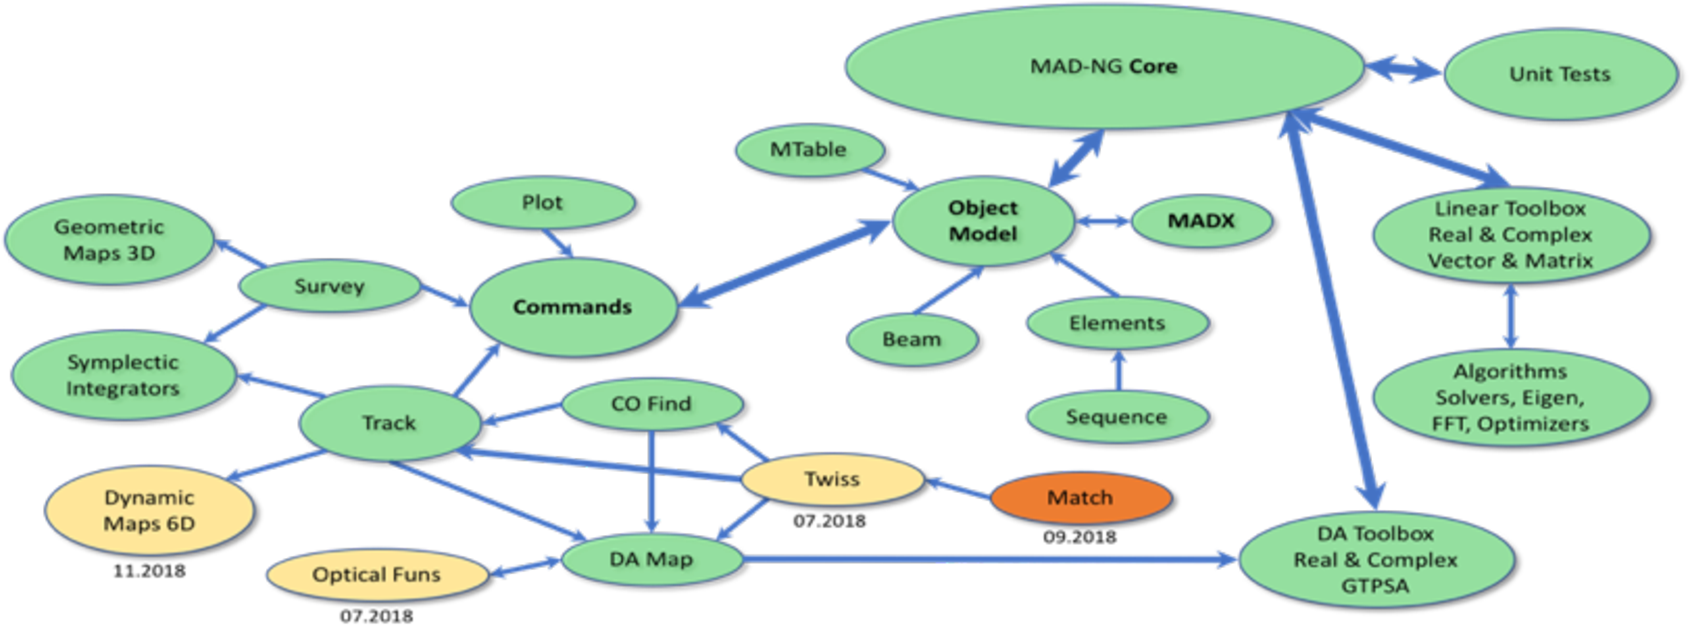
\includegraphics[width=\textwidth]{./Images/mad-graph.pdf}
    \caption{Current module hierarchy of MAD-NG}
    \label{fig:mad-graph}
\end{figure}

The two backbone modules are \emph{Object} and \emph{Commands}. The \emph{Object}
module is the one responsible for describing the object model use in MAD (see
Chapter \ref{Chapt:MO} for more). The \emph{Commands} is a special kind of
object that has the particularity of executing an \emph{exec} function
(different for each type of command) with the user provided parameters at the
time of definition.

The two main data-structures are \emph{MTable} and \emph{Sequence}.
\emph{Sequence} is used to represent particle accelerator inside of MAD.
It allows to build and edit them by
composition of different \emph{Element} with relative or absolute position.
\emph{Element} is the parent object of anything that can compose a
\emph{sequence} such as magnets (sbend, rbend, quadrupole, sextupole),
rfcavity or patch elements (translation, rotation, change of referential,
etc.). \emph{MTable} is a dynamic table structure that offers multiple
services, it grows and shrinks automatically, it can store heterogeneous data,
columns and lines can be access by name or indexes and column containing only
numbers are specialized to vectors to allow faster and more convenient
mathematical operations on them.

The core functionality of MAD comes from the provided high level \emph{Commands}.
The \emph{Survey} command computes the geometrical layout of a \emph{Sequence}.
It takes the initial parameters provided to calculate the coordinates of all
machine elements in a global reference system. The \emph{Track} command allows
to compute the evolution of a number of particles with given initial conditions
through a \emph{Sequence}, for one or many turns (to simulate ring-like particle
accelerator).